\justifying
\NSFCBodyText

\subsubsection{研究内容}

本项目围绕动态任务下智能体的持续后训练展开，研究对象为具有明确工具接口、状态转移和结果判定的文本工具智能体。四项研究内容分别考察参数更新、轨迹训练价值、历史能力保持和行动选择，形成由证据支持的持续适应过程。拟在公开模型与可复现沙箱上实现 PACT-Agent，研究任务分布变化、工具规则变化和反馈噪声三类干预，不将真实业务上线作为检验方法有效性的前提。

\textbf{研究内容一：动态任务感知的参数高效适配。}研究任务表征、可观察漂移证据与低秩参数更新收益之间的关系。任务表征由请求语义、所需工具、轨迹长度和历史失败类型构成；漂移检测仅使用当前可获得的任务输入与既往日志。针对新建、复用、冻结或调整适配器等候选动作，估计其单位计算成本下的适配收益与旧能力干扰，在预定总预算内选择更新位置和低秩容量。重点判断：任务变化能否提供超出梯度重要性本身的信息，以及这种信息在反馈噪声较高时何时失效。

\textbf{研究内容二：证据驱动的可信轨迹筛选与学习。}研究执行状态、验证器判断、轨迹一致性和模型不确定性对样本训练价值的共同作用。分别定义轨迹是否满足任务目标、是否包含可定位错误，以及加入训练后是否改善独立开发集表现。优先用确定性工具状态与约束检查建立标签，再以审计样本估计验证器偏差；对缺乏可靠结果的轨迹保留未知状态。形成面向监督微调、样本加权和同任务偏好对构造的选择机制，考察其能否在相同候选池和训练成本下保留有效困难样本、减少伪成功轨迹。

\textbf{研究内容三：有限记忆下的能力保持与持续后训练。}研究参数记忆和经验轨迹记忆在固定容量下的作用差异。参数记忆记录适配器的能力覆盖、版本与使用代价；轨迹记忆保留覆盖历史任务和典型失败类型的可验证样本。针对新任务学习引起的干扰，比较适配器复用、正交约束、经验重放和组合机制。对过期工具轨迹重新执行规则校验，必要时淘汰；通过预先保留的历史开发样本判断合并或替换是否可接受。目标是明确有限记忆条件下能够保留什么能力，以及何种任务差异会导致保持与适应之间的冲突。

\textbf{研究内容四：行动置信校准与风险感知执行。}研究候选动作的预测置信度与其实际正确性之间的对应关系，并与整项任务成功概率分别建模。以更新后冻结的策略在独立校准任务上生成动作，构造执行前可用的证据特征；在沙箱中获得动作后果标签，再建立校准器和选择规则。比较直接执行、追加验证、有限次重规划和拒绝四类行为，联合评估执行覆盖率、选择风险、全任务成功率和额外开销。重点分析策略改变、接口更新及标签延迟对校准器有效性的影响。

\subsubsection{研究目标}

总体目标是在固定训练与记忆预算下，建立可重现的 PACT-Agent 方法，解释证据条件如何改变新任务适应、历史能力保持和行动风险的关系。项目以可检验的方法与边界结论为成果，不将大模型规模增长或额外调用次数作为取得性能优势的主要来源。

参数适配以等预算任务成功率和适配速度为终点，对照静态 LoRA、AdaLoRA 及不更新策略；轨迹学习以同一候选池中的净训练收益、伪成功保留率和困难正确样本覆盖率为终点，对照随机选择、仅成功过滤及仅验证器选择；能力保持以固定记忆下的平均历史成功率和遗忘量为终点，对照仅重放、O-LoRA 与固定路由；行动校准以风险覆盖率曲线、Brier分数及全任务成功率为终点，对照未校准、温度缩放和固定阈值执行。各目标使用同一任务版本及共同随机种子配对比较。

\subsubsection{拟解决的关键科学问题}

\textbf{其一，任务变化如何转化为参数更新需求？}任务特征相近未必需要相同参数子空间，工具接口变化也可能仅需更新少量映射。项目比较任务证据和梯度重要性对候选更新收益的增量解释力，检验任务感知分配是否在预算匹配后仍有效。

\textbf{其二，什么证据能够识别真正有用的学习轨迹？}结果正确、步骤正确与训练有益是不同属性。项目分析不确定性与执行证据是否存在互补作用，特别考察验证器与生成器错误相关时的失效，以及高质量筛选是否损害长尾任务覆盖。

\textbf{其三，能力保持与行动校准何时能够兼容？}旧任务正确率恢复后，置信度仍可能偏移；保护历史参数也可能妨碍新工具适应。项目在相同策略版本下分别测量遗忘和校准误差，并检验独立校准对降低行动风险的贡献及其成本。

\subsubsection{研究方法}

\textbf{问题形式化与资源约束。}设第 $t$ 阶段的任务分布为 $\mathcal{D}_t$，冻结主干参数为 $\theta_0$，可训练低秩参数为 $\phi_t$，记忆为 $\mathcal{M}_t$，校准器为 $g_t$。一条轨迹记为 $\tau=(x,a_1,o_1,\ldots,a_K,o_K,y)$，其中 $x$ 为任务，$a_k$ 与 $o_k$ 分别为动作和工具观测，$y$ 为经任务判定器核验的结果。未能判定的 $y$ 不当作成功标签。拟采用如下受约束目标组织比较：
\begin{equation}
\max\ \overline{S}\quad
\text{s.t.}\quad F\leq\delta_F,\quad R(c_0)\leq\delta_R,\quad
P_{\mathrm{all}}\leq B_P,\quad |\mathcal{M}_t|_{\mathrm{byte}}\leq B_M,\quad C_{\mathrm{all}}\leq B_C .
\end{equation}
这里 $\overline{S}$ 为按阶段等权平均的任务成功率，每阶段以全部指派任务为分母，拒绝与未完成不计成功。$F$ 为历史任务遗忘量：在各历史任务、原工具及判定器的冻结快照上，以该任务学习结束时的策略为参照，计算当前策略成功率降幅的非负部分并对历史任务等权平均；现行规则下的迁移成功率另报，不混入 $F$。$R(c_0)$ 为预定覆盖率 $c_0$ 下的选择风险。$P_{\mathrm{all}}$ 统计所有保留适配器、路由器及新增预测模块，$C_{\mathrm{all}}$ 包括轨迹生成、验证、探测更新、正式训练和重新校准的实际成本，调参、审计及失败运行逐方法列账，共用评价成本单列；外部调用费用另列。$\delta_F$、$\delta_R$ 与 $c_0$ 在开发阶段预先锁定。若约束不可同时满足，报告不可行区域及各项代价，不以改变阈值隐藏失败。

\textbf{数据来源与任务变化。}主要采用 AgentBench 中可离线运行的文本交互任务和 $\tau$-bench 的工具与末态判定思想构建版本化实验；现有标准测试集作为冻结外部评价，定制训练任务另行生成并审计\cite{agentbench,taubench}。工具沙箱实现检索、计算、结构化查询和受控状态修改等能力，所有状态修改限定在可重置实验副本。分别设置任务组成渐变、工具字段或规则突变、反馈错误及延迟，再设置少量复合变化。每类变化都记录实际操作和标签生成方式，避免把增加题目难度直接等同于分布漂移。

公开能源时序数据作为第二层验证，智能体完成历史窗口读取、预测器选择、误差计算与报告生成。以训练时可见的时间戳为界构造季节变化和噪声变化，预测目标仅在其真实可获得时点进入反馈。数据具体来源与许可在首阶段核验后固定，不声称已取得私有场站或电网数据。该环境用于检验方法对非平稳任务的适用性，不把金融交易收益或真实电网控制作为终点。

\textbf{训练、调参与评价隔离。}主实验在每个已发生的工具版本内，按独立任务来源、模板与用户意图划分训练集、开发集、校准集和最终测试集，并遵守反馈时间先后；版本作为共同实验条件，同源任务不跨区。完全未见版本的外推评价另列，在获得该版本反馈前不得重校准。同源任务的改写、同一状态派生轨迹和近重复问题放在同一分区。开发集用于预算选择、质量分学习和超参数比较；校准集只在策略冻结后拟合概率映射与执行门槛；测试集用于阶段性冻结评价，结果不回流算法。另设可重放的历史开发样本判断适配器合并，不能借助历史测试集选择保留哪一个模型。开发任务再按模板交叉留出，质量分拟合与效用预测核验使用不同折；历史校准记录仅在对应版本的校准比较中使用，不转作训练或质量分拟合样本。

实验规模初稿为\textbf{【暂定：以3B级模型完成主实验，7B级模型完成关键复核；设置6个连续任务阶段、3种任务顺序和3个训练随机种子】}。每阶段样本量先通过小规模试跑估计成本，再在正式比较前锁定。全参数微调仅作为可承受规模的参照，超过统一预算时报告其成本及不可比部分。主要效果比较使用等GPU时方案，并补充等训练样本与等可训练参数方案，避免用单一“参数少”替代实际效率。

\textbf{统计分析与失败判据。}以任务实例为配对单位汇总成功和失败，以任务模板或时间块为重采样簇，报告成功率差、遗忘量差及风险覆盖率曲线的置信区间。随机种子作为重复实验单独呈现，不将同一轨迹中的多个步骤当作独立样本。预先指定一个主要比较：在锁定覆盖率、遗忘和风险容限下，完整方法相对最强等预算组合基线的任务成功率差。最强组合基线及阶段权重在开发阶段确定，不由测试结果反选。

最小有效成功率收益 $\epsilon_S$ 以及绝对遗忘、风险容限 $\delta_F$、$\delta_R$ 在开发阶段锁定。支持主要假说要求成功率差置信区间下界超过 $\epsilon_S$，且完整方法的 $F$、$R(c_0)$ 区间上界分别不超过 $\delta_F$、$\delta_R$；成功率差上界低于 $\epsilon_S$，或 $F$、$R(c_0)$ 的区间下界超过对应容限时构成反证，其余情况报告证据不足。遗忘差另作次要比较，不混入绝对容限的判据。多条路线的次要检验采用多重比较校正。结果分析同时保留失败任务与不可判定结果，避免只分析被系统接受的轨迹。

执行覆盖率定义为至少执行一次动作的任务数占全部指派任务数，选择风险定义为至少出现一次错误执行的任务数占有执行任务数；中途拒绝的任务仍计入相应分母。同时报告最终完成率、执行步数和最大步数，防止提前停止造成表面改善。覆盖容差在开发阶段锁定，测试报告实际覆盖；无法达到预定覆盖率时记为不可达，不外推风险值。预先固定动作结果观察窗口：已确认错误的任务计入错误数；尚无已知错误但存在未知动作结果的任务单列为未知。风险识别下界为已知错误数除以执行任务数，上界为已知错误与未知任务数之和除以执行任务数，同时报告未知率。风险区间同时包络识别上下界与抽样不确定性：支持风险约束须使保守上界的抽样上限低于容限，反证则须已知错误下界的抽样下限超过容限；仅因未知率高而上界超限时报告证据不足。概率评分只评价结果可判定的动作并报告标签覆盖，未知结果不视为正确。

\subsubsection{技术路线}

\textbf{总体技术路线。}先固定任务、工具和评价版本，用既往交互记录构造任务状态与漂移证据；据此选择低秩更新的候选位置和预算，再由当前策略生成训练轨迹。轨迹经独立执行检查、验证器及一致性检查后进入质量建模，为参数更新和记忆选择提供依据。完成有界记忆约束下的持续后训练后，冻结新策略，使用独立校准任务确定动作概率映射和选择门槛。部署于沙箱的策略产生新日志，只有在下一轮划分中允许使用的记录才能进入后续训练，最终测试结果始终隔离。四条分路线由此共享证据定义和接口，各自使用符合用途的数据分区。
% NSFC-ILLUSTRATED BEGIN F02
如图~\ref{fig:pact-f02} 所示，PACT-Agent总体研究框架。四路线共享证据定义与接口，训练、开发、校准和测试记录按用途隔离；所有适配器及证据获取成本均计入累计预算。
\begin{figure}[htbp]
\centering
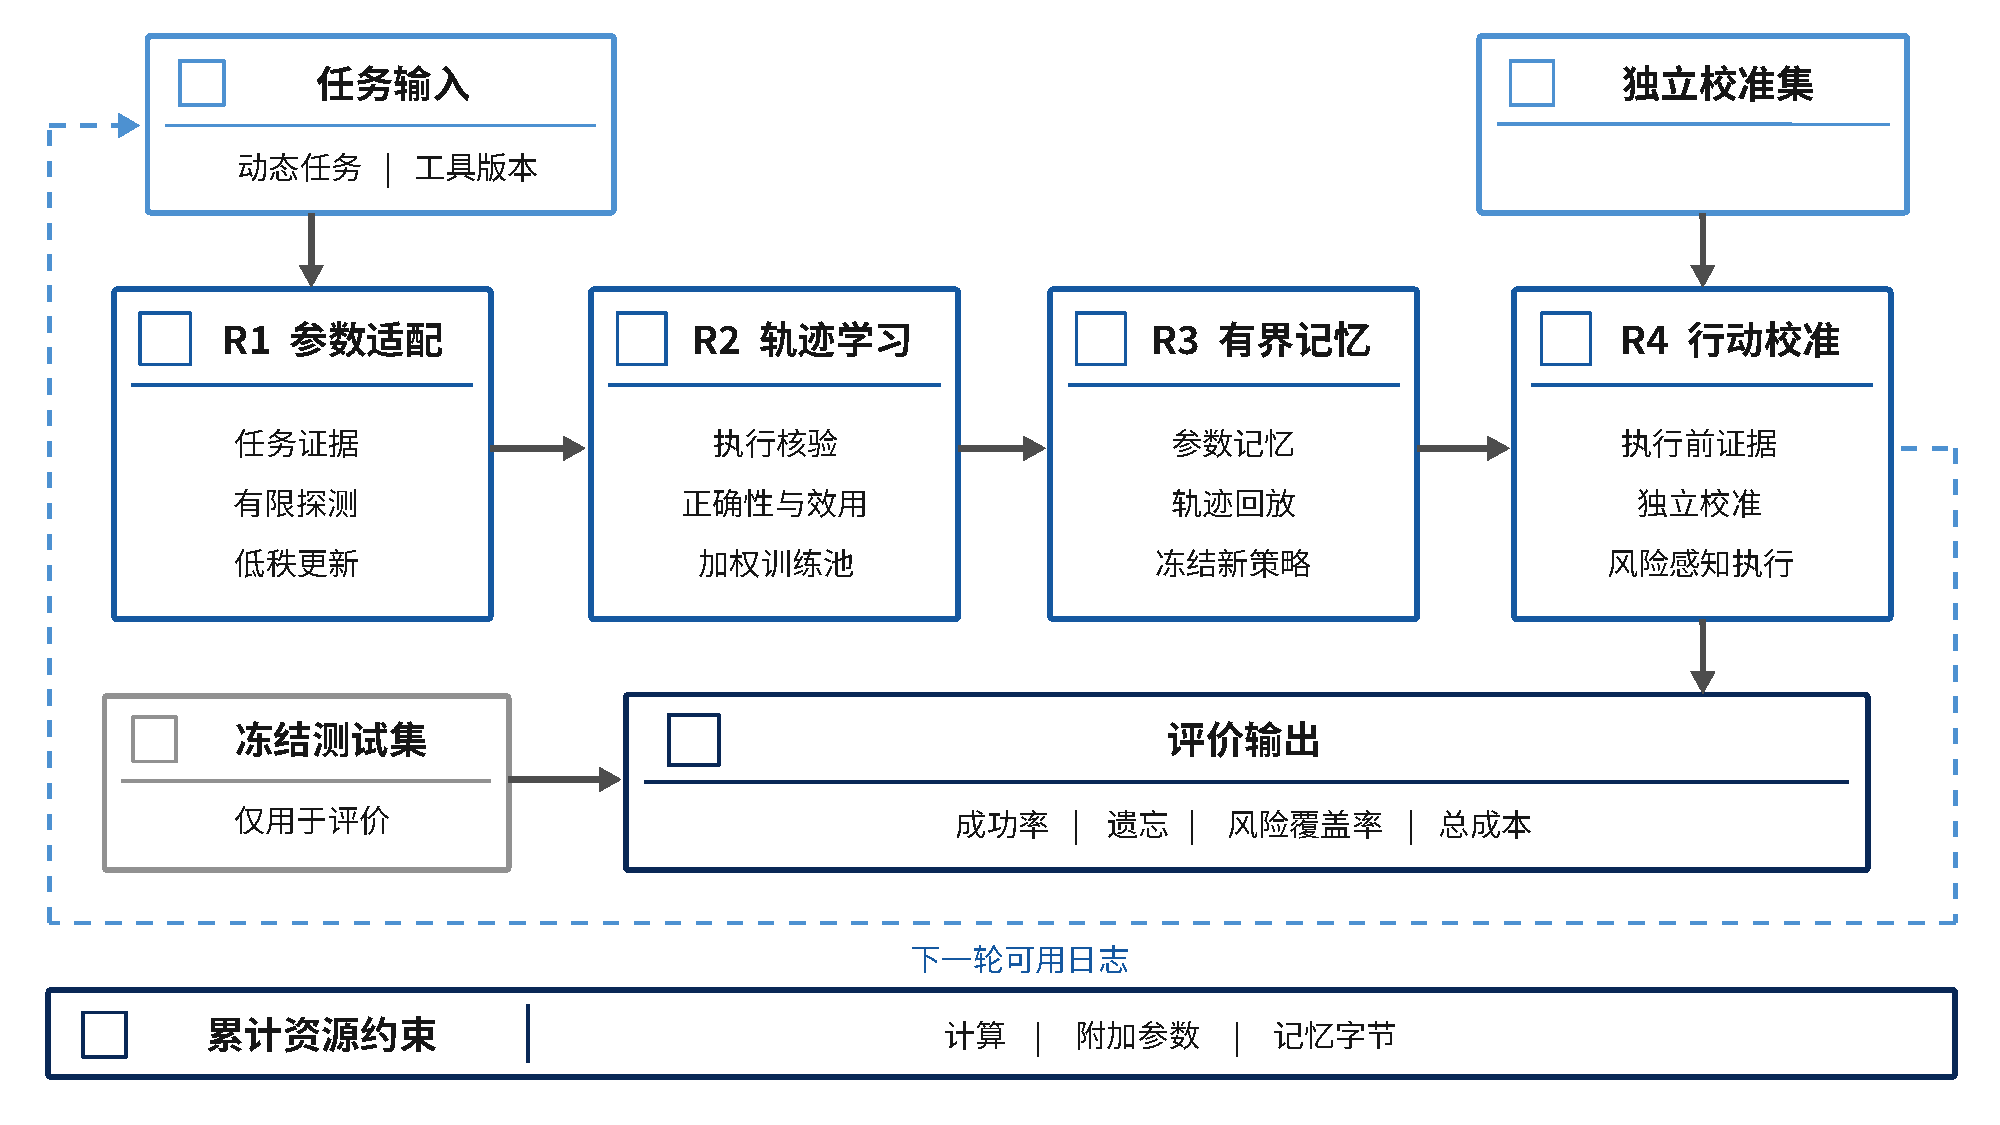
\includegraphics[width=1\linewidth]{figures/F02.pdf}
\caption{PACT-Agent总体研究框架。四路线共享证据定义与接口，训练、开发、校准和测试记录按用途隔离；所有适配器及证据获取成本均计入累计预算}
\label{fig:pact-f02}
\end{figure}
% NSFC-ILLUSTRATED END F02


\textbf{分路线一：任务感知的参数高效适配。}输入当前任务特征、过去阶段的训练日志、适配器摘要及剩余预算。首先将请求语义、工具集合和既往失败类别编码为任务状态 $z_t$，以窗口比较得到漂移证据 $d_t$；再在预定低秩配置集合中进行有限次探测更新，估计不同层与适配器的开发集收益及历史开发集损失。探测成本计入总预算，既往轨迹尚未获得标签时不使用未来结果。以候选更新的收益与成本比排序，并施加总容量限制，在复用、更新、冻结和替换之间选择；不会无限追加适配器。输出带有版本和成本记录的适配策略，为轨迹生成提供当前 Agent。与静态 LoRA、AdaLoRA 和随机任务路由比较，并打乱任务证据但保持计算量不变，以判断收益是否确由任务信息带来\cite{lora,adalora}。
% NSFC-ILLUSTRATED BEGIN F03
如图~\ref{fig:pact-f03} 所示，路线一：依据任务与历史开发证据，在累计容量和计算预算内选择复用、更新、冻结或替换。有限探测计入总成本，历史测试结果不参与决策。
\begin{figure}[htbp]
\centering
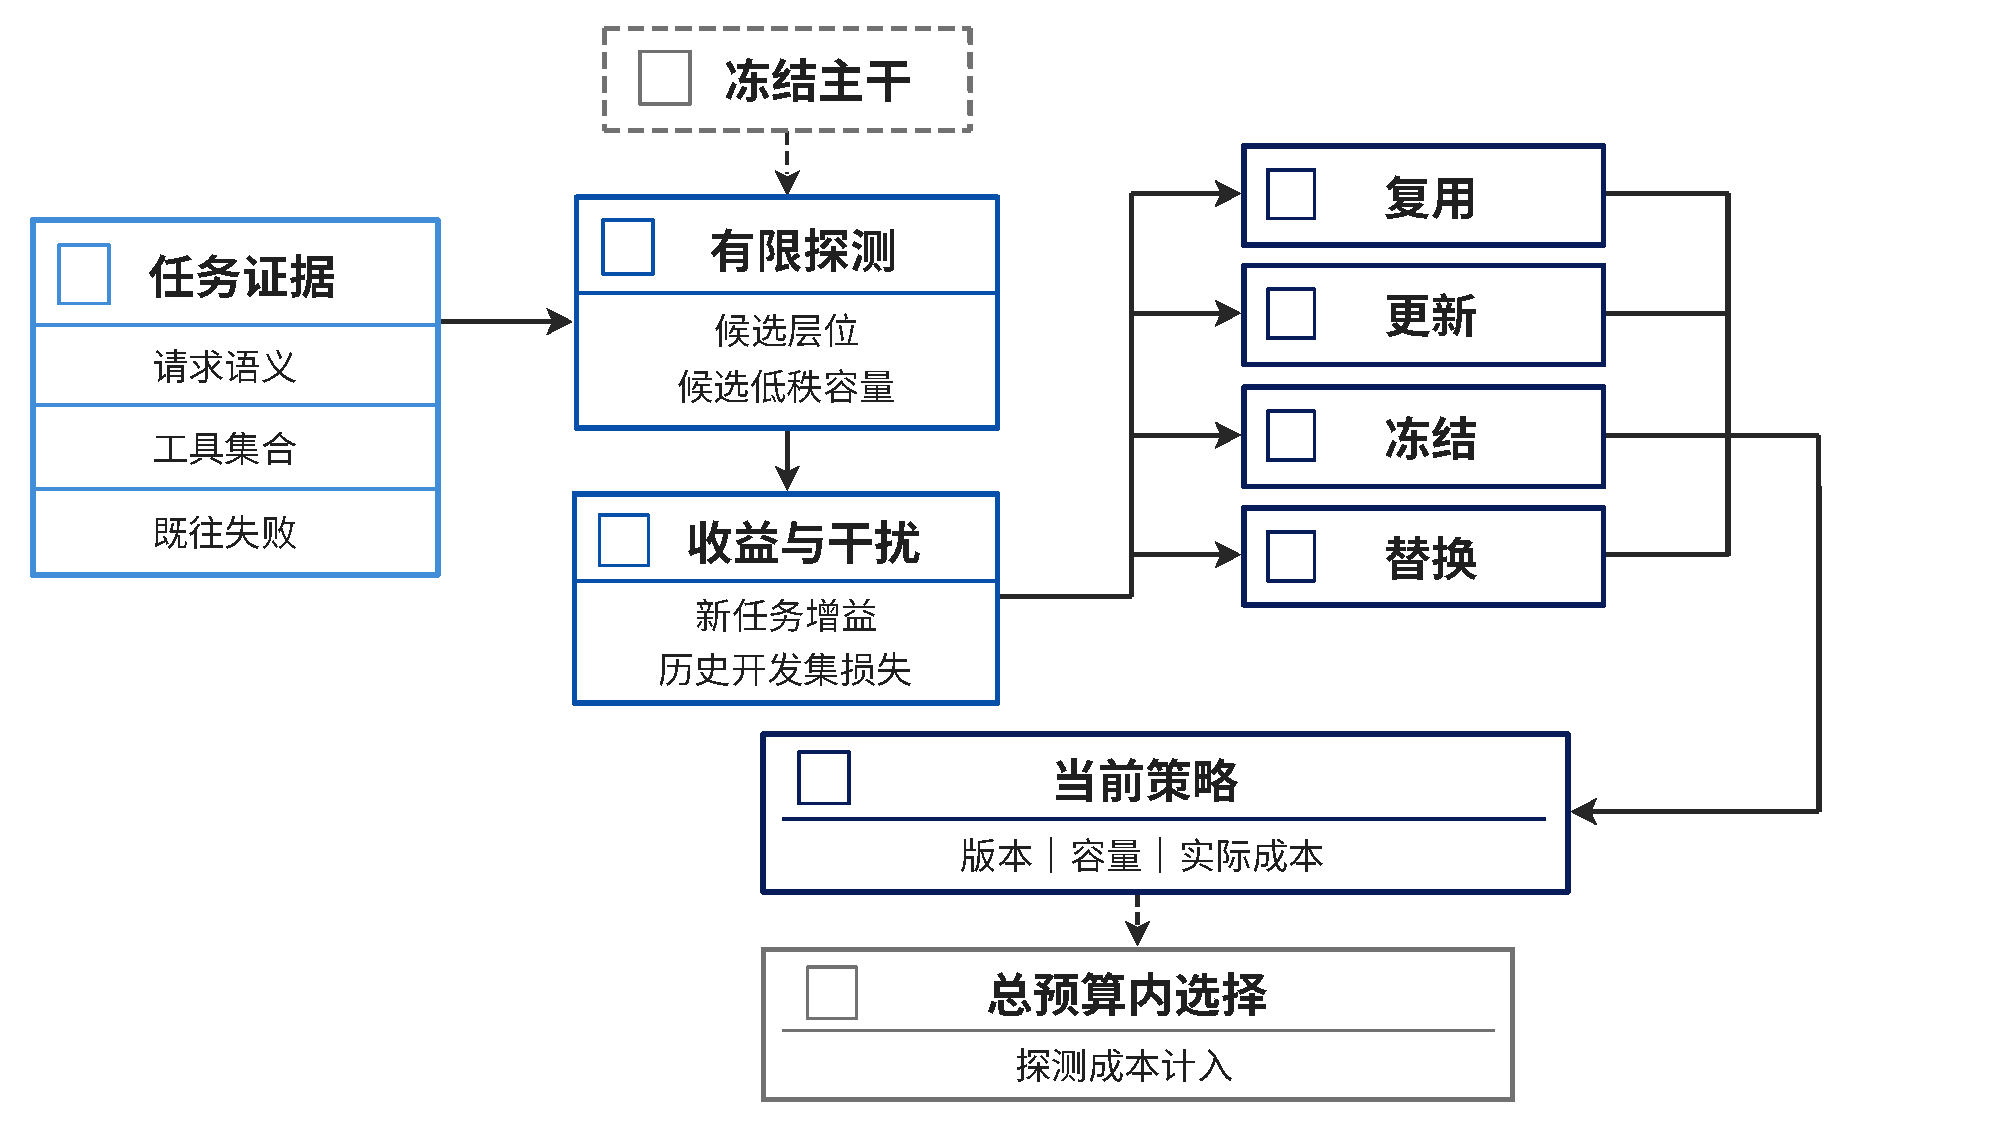
\includegraphics[width=1\linewidth]{figures/F03.pdf}
\caption{路线一：依据任务与历史开发证据，在累计容量和计算预算内选择复用、更新、冻结或替换。有限探测计入总成本，历史测试结果不参与决策}
\label{fig:pact-f03}
\end{figure}
% NSFC-ILLUSTRATED END F03


\textbf{分路线二：证据驱动的可信轨迹学习。}输入路线一产生的候选轨迹及工具版本。先由末态目标、参数合法性和任务约束给出执行证据 $e$，再加入验证器分数 $v$、轨迹一致性 $s$ 和不确定性 $u$。以人工抽查和确定性标签构成的开发数据学习质量分 $q=f(e,v,s,u)$，分别保留正确性估计和训练效用估计，不将 $q$ 直接解释为成功概率。对无结果标签的轨迹设置未知类别；对困难但已验证正确的样本维持覆盖配额。监督训练使用有界权重，偏好训练只对同任务、相近工具成本且优劣有独立证据的轨迹配对，防止较长轨迹仅因调用更多而被判优\cite{dpo,agenttuning}。输出加权训练池、可信偏好对和审计记录，交给路线三完成更新与记忆管理。验证时固定候选池，对照随机、成功过滤、单验证器及全部证据方案。训练效用以配对短程探测中“加入／不加入同一轨迹”对独立开发任务的增量收益为依据，候选模型、训练步数及随机种子配对；验证器标签不能同时充当该效用的真值。
% NSFC-ILLUSTRATED BEGIN F04
如图~\ref{fig:pact-f04} 所示，路线二：分开判断轨迹正确性和增量训练效用。配对短程探测的收益来自独立开发任务；未知轨迹保留待审，不视作成功样本。
\begin{figure}[htbp]
\centering
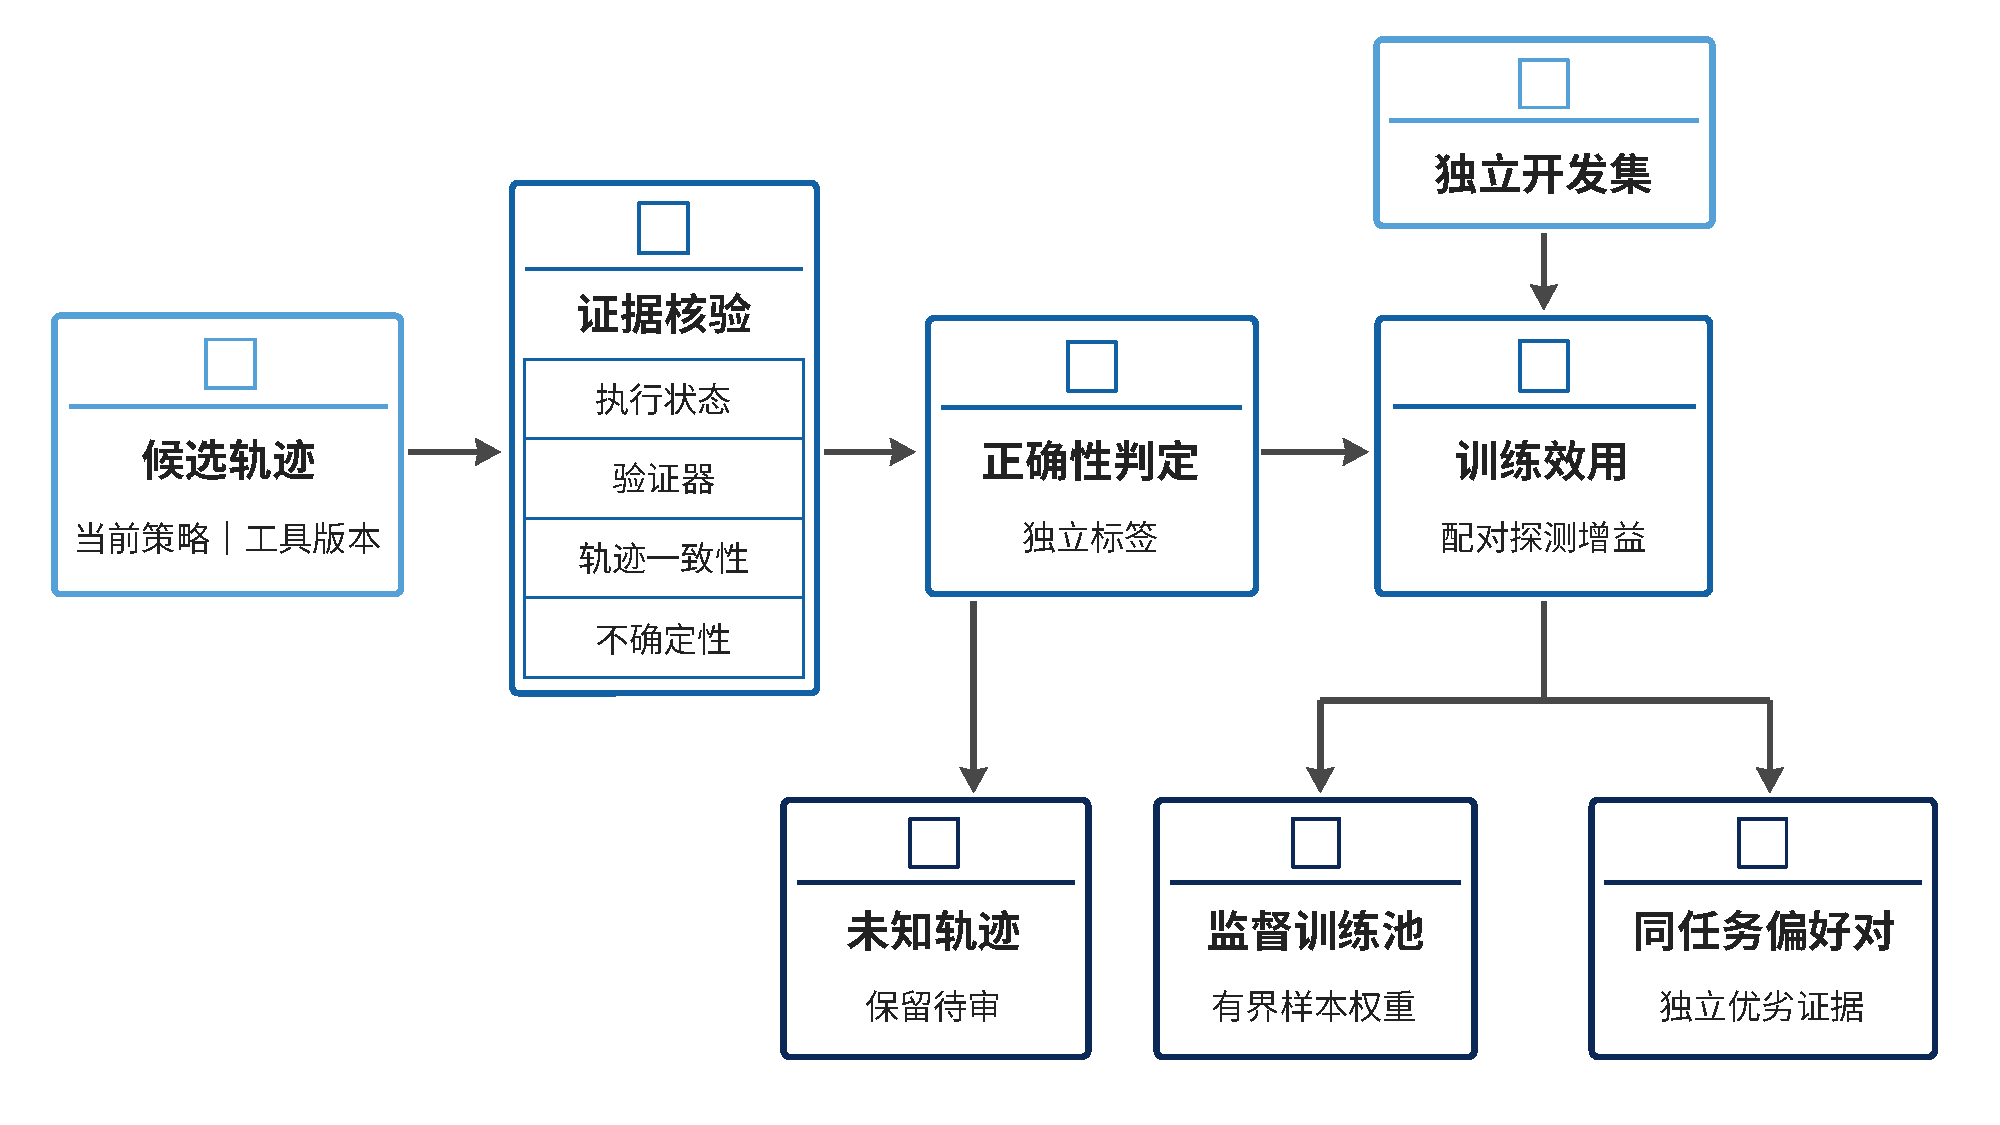
\includegraphics[width=1\linewidth]{figures/F04.pdf}
\caption{路线二：分开判断轨迹正确性和增量训练效用。配对短程探测的收益来自独立开发任务；未知轨迹保留待审，不视作成功样本}
\label{fig:pact-f04}
\end{figure}
% NSFC-ILLUSTRATED END F04


\textbf{分路线三：有界记忆下的持续抗遗忘。}输入加权训练池、历史适配器及轨迹记忆。以覆盖任务能力和失败类型为原则选择固定字节容量的回放样本，并剔除已不符合当前工具规则的记录。更新目标由当前任务学习项、历史重放项和低秩干扰约束组成；先采用固定权重作为基线，再比较由开发集证据控制的有限候选权重。参考 O-LoRA 对参数子空间干扰的处理，并以 GEM 式历史约束作为方法参照\cite{olora,gem}。适配器库达到容量上限时，根据历史开发集表现决定合并、替换或冻结，合并失败则保留旧版本并缩减新任务目标。输出固定容量的适配器库、经验记忆及冻结后的策略版本，随后交给路线四校准。消融分别关闭参数记忆、轨迹记忆和证据协调，保持容量、训练步数及回放读取量匹配，以识别两类记忆的作用及交互。
% NSFC-ILLUSTRATED BEGIN F05
如图~\ref{fig:pact-f05} 所示，路线三：在附加参数和轨迹字节容量限制下联合管理参数记忆与经验回放。合并选择依据历史开发集，历史测试集仅报告能力保持结果。
\begin{figure}[htbp]
\centering
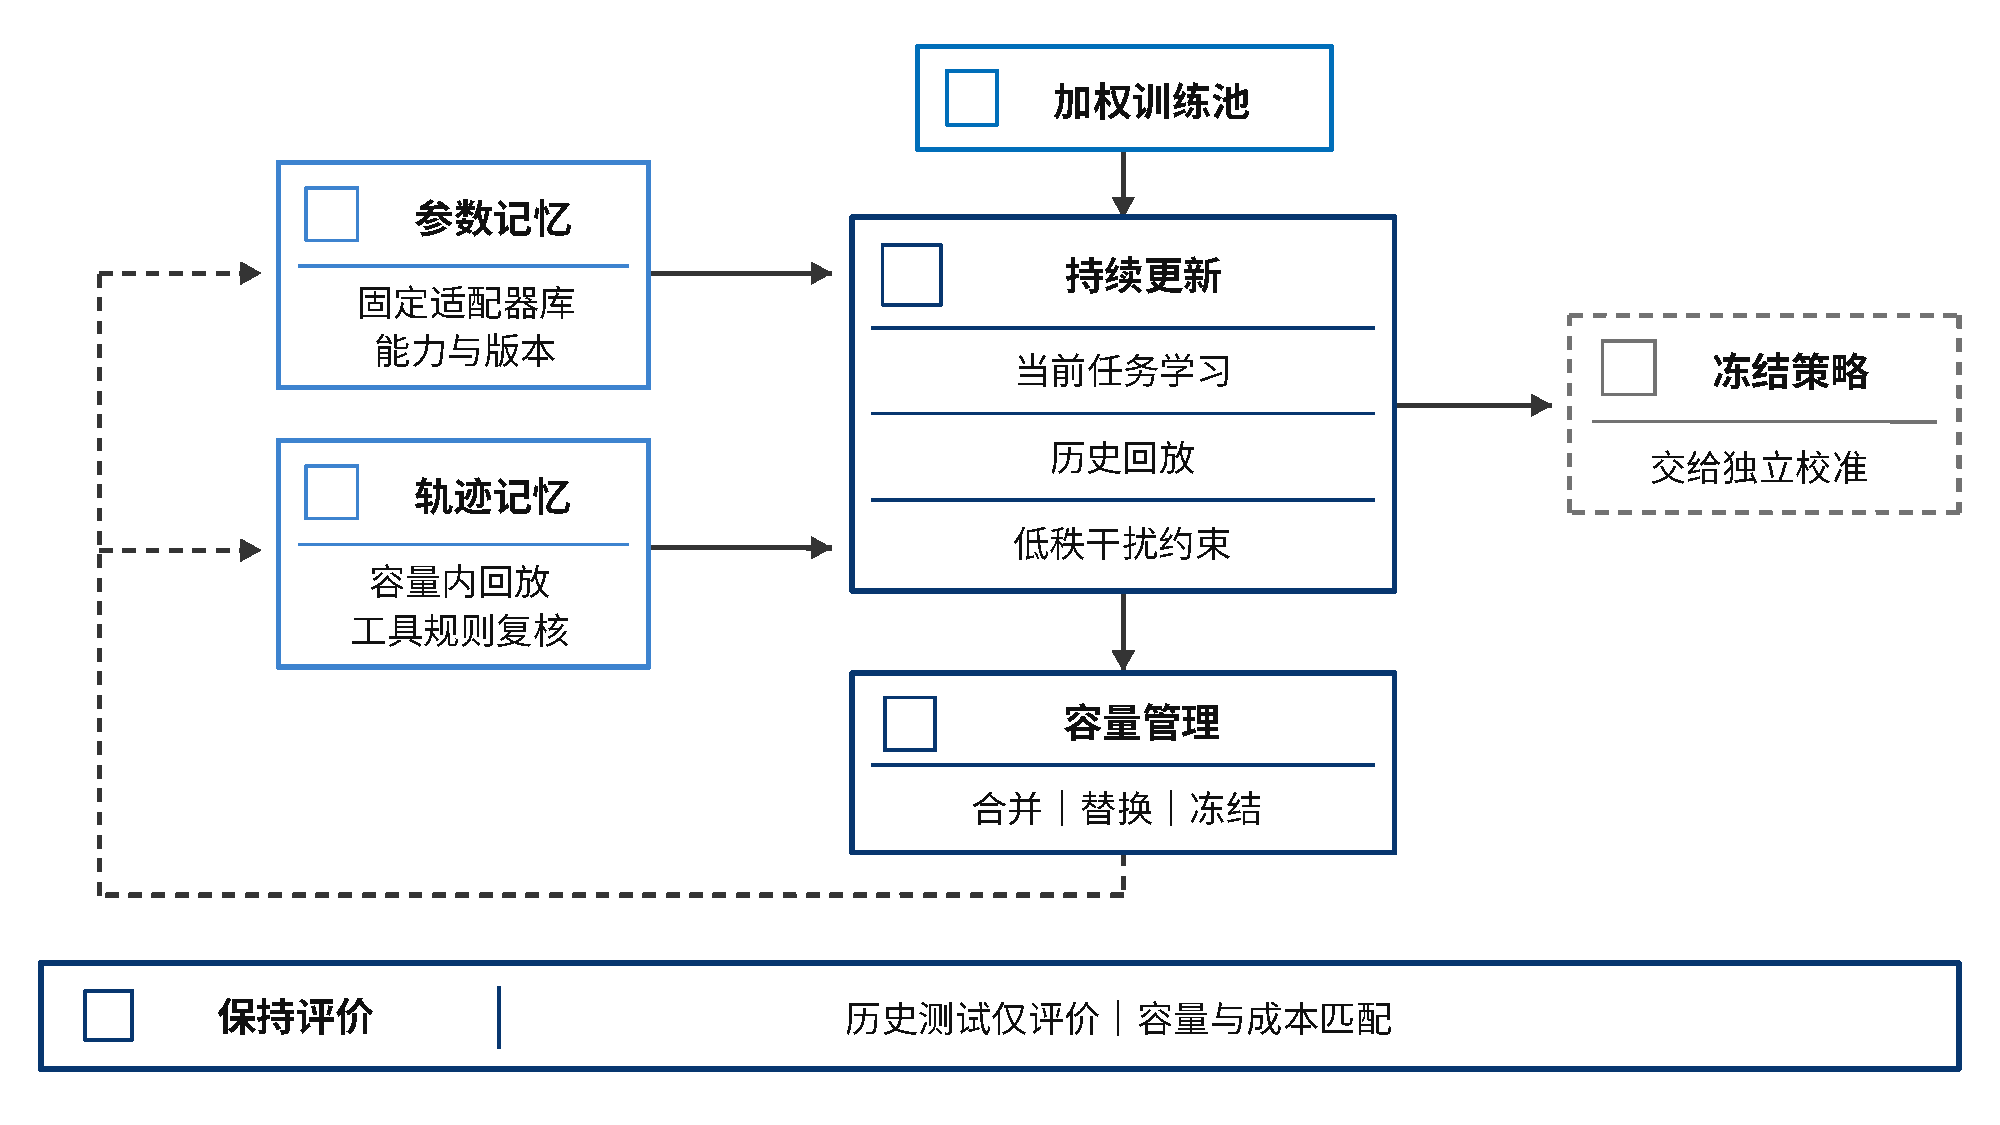
\includegraphics[width=1\linewidth]{figures/F05.pdf}
\caption{路线三：在附加参数和轨迹字节容量限制下联合管理参数记忆与经验回放。合并选择依据历史开发集，历史测试集仅报告能力保持结果}
\label{fig:pact-f05}
\end{figure}
% NSFC-ILLUSTRATED END F05


\textbf{分路线四：独立校准与风险感知执行。}输入冻结策略、当前工具版本和独立校准任务。对动作 $a$ 仅使用执行前的上下文、模型输出及已观察历史构造特征 $h$，预测其正确性 $p=g(h)$；另为整项任务成功建立单独预测头，避免两种概率混淆。以温度缩放或逻辑校准为基础，比较加入漂移和工具状态特征后的校准效果\cite{calibration}。对同一标量动作正确性分数采用单调温度缩放，作为保持排序的校准对照，其 Brier 分数改善不能直接证明同覆盖率风险降低；后者只检验新增行动证据是否改善选择排序。对每个候选动作按预定门槛选择执行、追加验证、有限重规划或拒绝，所有追加操作计入推理成本。校准任务中的候选动作在可重置副本上获得影子结果，主执行是否接受不影响其被评估机会，从而缓解只观测已接受动作的偏差。该影子过程仅用于沙箱评价，不推定真实业务中可获得反事实标签。输出校准器、阈值及风险覆盖率结果，分别检验冻结校准、每阶段重校准和漂移触发重校准。反馈不足或工具规则突然改变时转为保守执行并记录覆盖率下降，不声称无条件风险保证\cite{selective,conformalrisk,adaptiveconformal}。
% NSFC-ILLUSTRATED BEGIN F06
如图~\ref{fig:pact-f06} 所示，路线四：冻结策略后独立校准，并根据执行前可用证据选择行动。影子标签仅用于可重置沙箱中的校准和审计；概率评分与同覆盖率任务风险分别评价。
\begin{figure}[htbp]
\centering
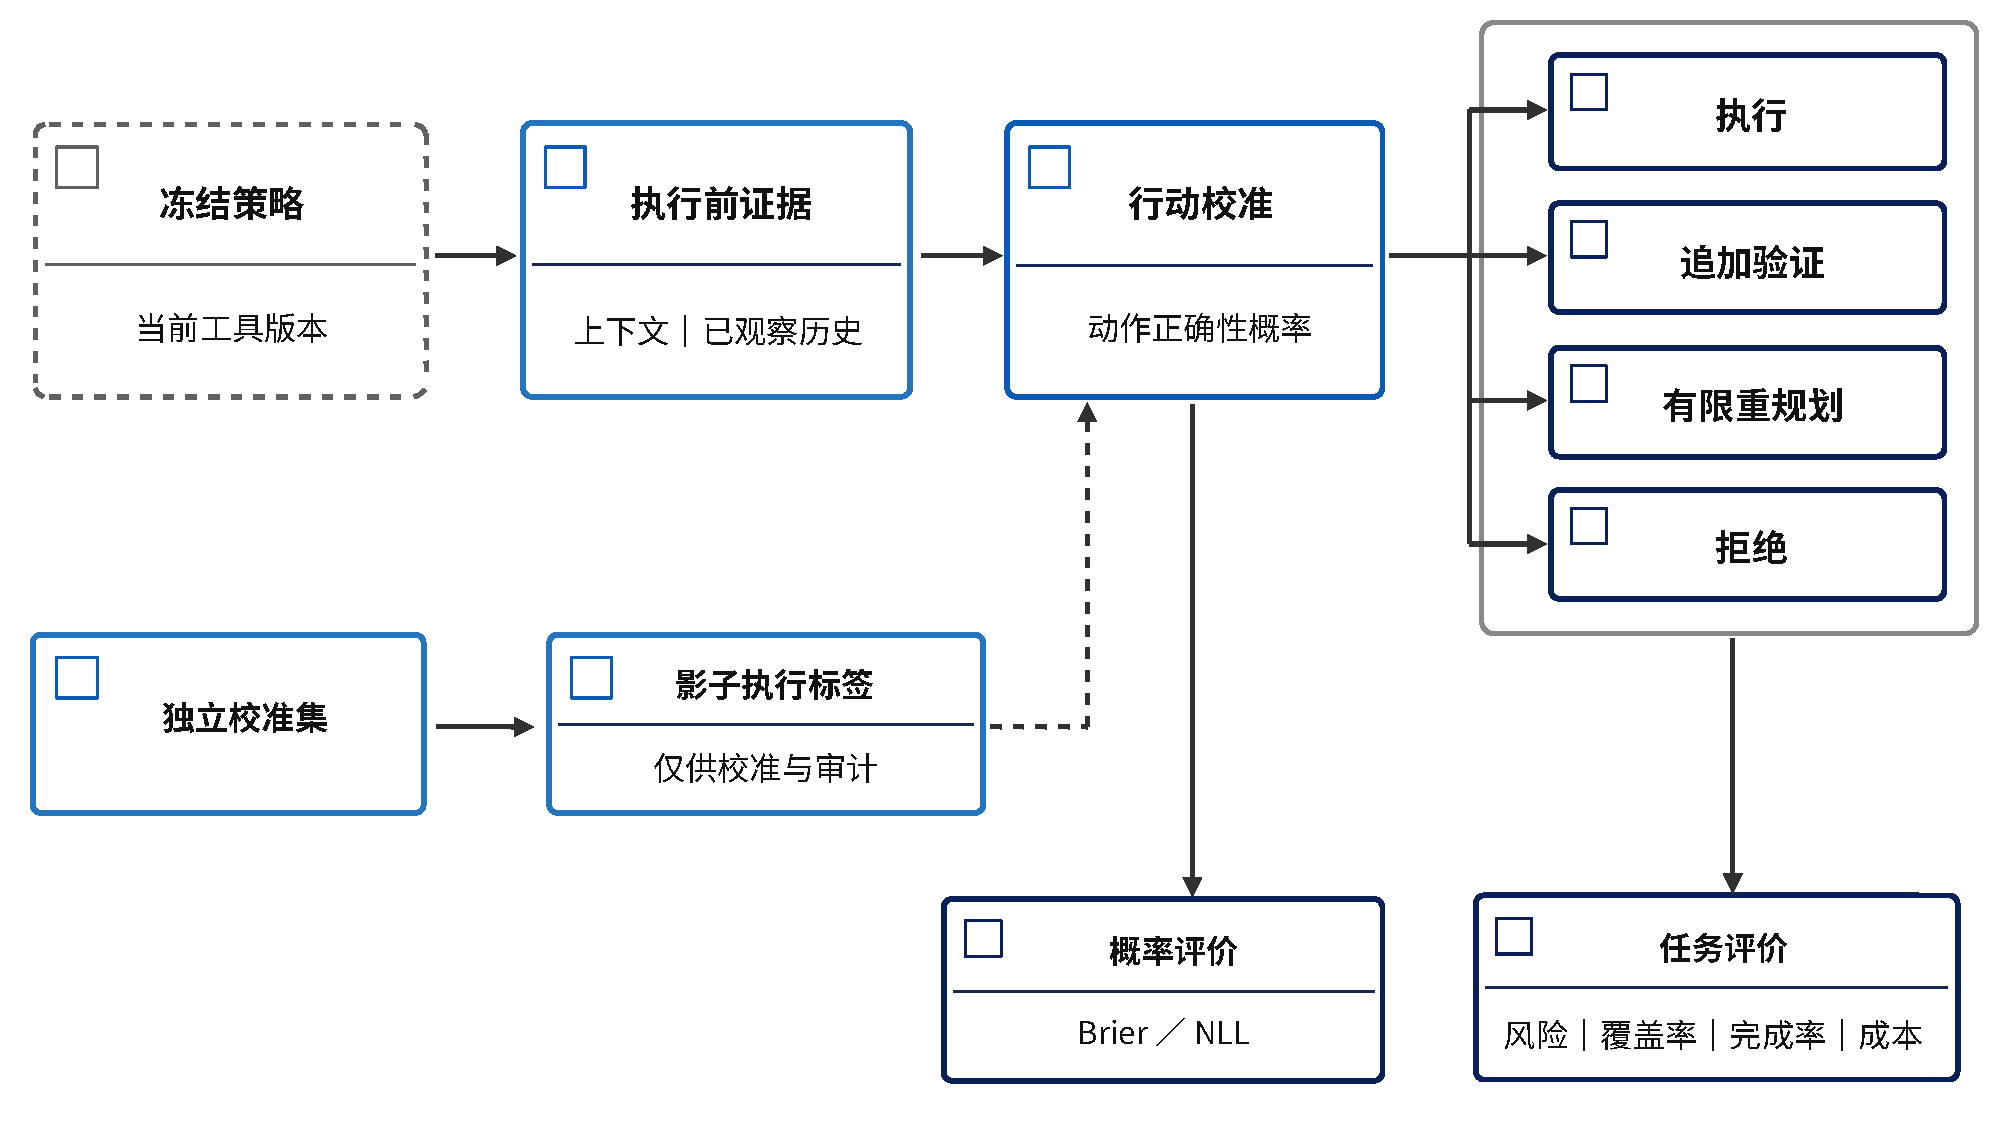
\includegraphics[width=1\linewidth]{figures/F06.pdf}
\caption{路线四：冻结策略后独立校准，并根据执行前可用证据选择行动。影子标签仅用于可重置沙箱中的校准和审计；概率评分与同覆盖率任务风险分别评价}
\label{fig:pact-f06}
\end{figure}
% NSFC-ILLUSTRATED END F06


\subsubsection{关键技术}

\textbf{跨模块证据的一致表达。}为任务版本、工具版本、动作、观测、验证结果、模型版本和时间戳建立统一定义，使一条轨迹能够追溯其使用目的。共用的是变量含义与处理接口，训练轨迹和校准任务仍分别保存。对不确定性使用固定采样预算，分别比较输出概率、候选动作分歧和语义一致性；语义一致性仅辅助判断，最终以工具结果和任务约束区分等价动作\cite{semantic}。

\textbf{相关错误的机制对照。}在可确定真值的沙箱中设置“错误相关性高／低”与“错误轨迹回放剂量高／低”的 $2\times2$ 对照。按任务难度分层固定生成器及验证器的边际假阳性、假阴性率，预先锁定联合错误注入与多证据聚合规则，并固定任务重叠度。减少已知错误轨迹回放时，以任务、难度和长度匹配的正确轨迹补足训练量，使总训练成本相当。依次观察伪成功入选率、错误回放暴露量、参数干扰及历史任务损失，检验错误是否在低秩更新场景中被放大。真值替换仅用于机制诊断，不作为可部署算法的收益。若剂量干预未改变历史损失，或成本匹配后效应消失，则不支持该链式解释。
% NSFC-ILLUSTRATED BEGIN F07
如图~\ref{fig:pact-f07} 所示，实验隔离与机制对照示意。按任务来源和时间分区；相关错误与回放剂量构成2×2干预，分层匹配边际错误率、任务难度和训练量，图中不含实验结果。
\begin{figure}[htbp]
\centering
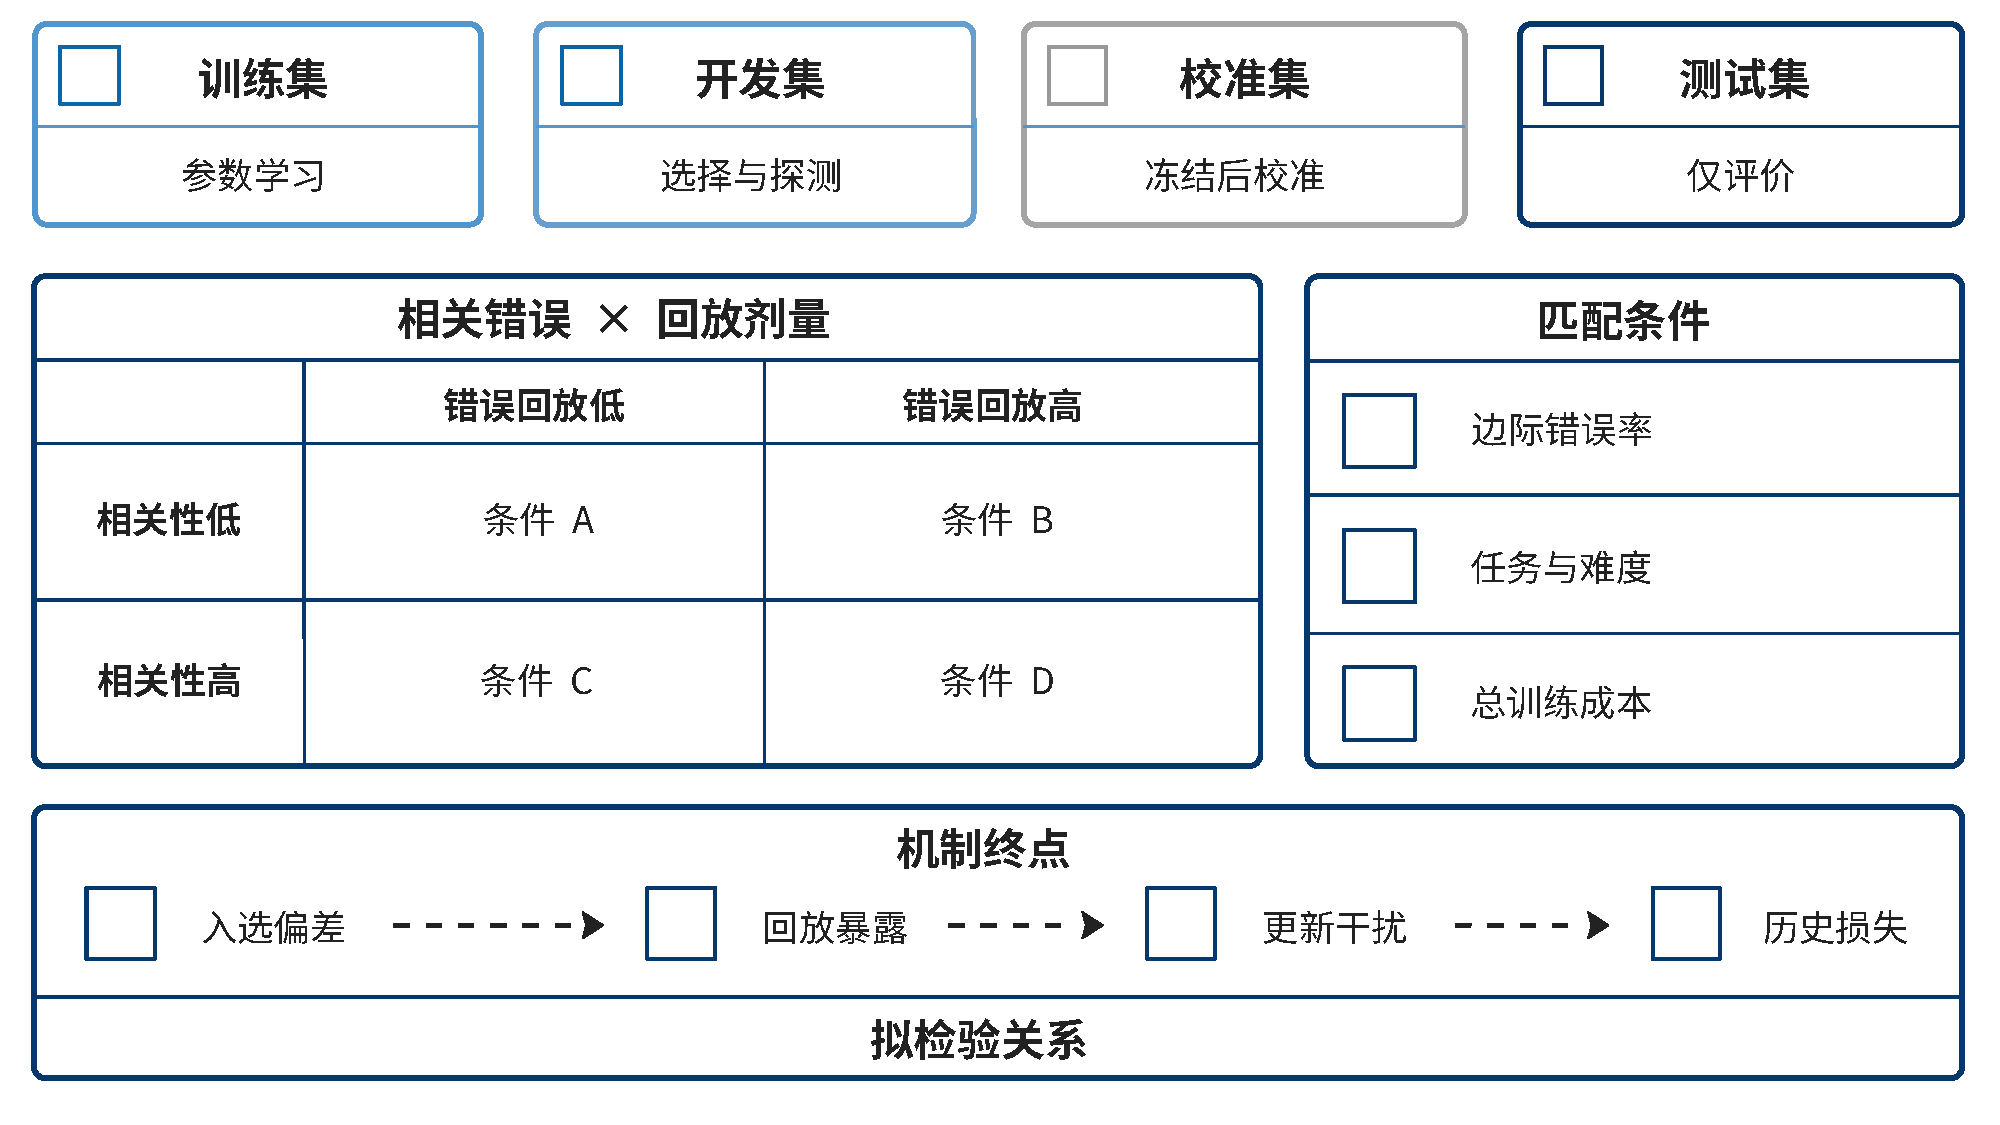
\includegraphics[width=1\linewidth]{figures/F07.pdf}
\caption{实验隔离与机制对照示意。按任务来源和时间分区；相关错误与回放剂量构成2×2干预，分层匹配边际错误率、任务难度和训练量，图中不含实验结果}
\label{fig:pact-f07}
\end{figure}
% NSFC-ILLUSTRATED END F07


\textbf{可识别的联合效果。}完整方法之外设置各模块获得同类证据、采用同类校准器并享有相同调参总预算的模块组合基线，仅关闭跨模块协调规则；删除或打乱证据另作信息消融。采用局部交互对照：轨迹筛选有无与记忆协调有无组成一组，策略更新有无与重校准有无组成另一组。在相同资源下检验交互项，避免将多个单模块改进简单相加后称为协同。主要对照均锁定工具、提示、解码与最大行动步数，必要时同时报告关闭重规划后的模型本体结果。

\textbf{跨框架复现与工程交付。}先实现最小可运行文本工具流程，保存低秩参数、日志及评价脚本，再完成飞桨生态兼容验证。跨框架迁移分别检查权重形状、分词与工具格式、固定输入输出差异及任务结果，尚未验证的功能不标为已兼容。参考 Agent Lightning 的训练与执行分离方式组织接口，但算法结论不依赖某一运行控制器的专属特性\cite{lightning,lightningv1}。

\subsubsection{可行性分析}

四条路线均具有可运行的基础对照：低秩适配、结果验证、经验回放与后处理校准可以先独立运行，再比较协调机制。某一路线未达到预期时，仍可通过独立对照形成清楚的边界结论。现有算力适合以中小规模开源模型开展参数高效实验；模型规模升级安排在关键机制得到证据之后。通过公开任务与自包含工具沙箱降低外部接口变更的影响，通过固定时间块与工具版本支持时序补充验证。首年优先完成可信对照和成本核算，扩展环境与更大模型根据阶段结果推进。
